%%%%%%%%%%%%%%%%%%%%%%%%%%%%%%%%%%%%%%%%%%%%%%%%%%%%%%%%%%%%%
%% Begin exercise %%
%%%%%%%%%%%%%%%%%%%%%%%%%%%%%%%%%%%%%%%%%%%%%%%%%%%%%%%%%%%%%
\ex{Fourier analysis of rotating fields}


\normalsize{\textbf{Acknowledgement}: The following exercise is adapted from ``Geregelte Drehstromantriebe / Controlled AC Drives'' by J. Böcker, Paderborn University, 2021 and 
``Elektrische Maschinen und Antriebe Übungsbuch: Aufgaben mit Lösungsweg'' by A. Binder, Springer, 2017
}\\



%%%%%%%%%%%%%%%%%%%%%%%%%%%%%%%%%%%%%%%%%%%%%%%%%%%%%%%%%%%%%
%% Task 1 %%
%%%%%%%%%%%%%%%%%%%%%%%%%%%%%%%%%%%%%%%%%%%%%%%%%%%%%%%%%%%%%

\task{Fourier analysis of a field distribution of a three-phase winding}
The winding of a three-phase and four-pole machine is described with the following parameters. The number of notches is given with $q$ = 2 and the winding chording is $y/\rho_{\mathrm{p}}$ = 5/6. The number of windings per coil is given with $N_{\mathrm{c}}$ = 5 with $a$ = 1. The air gap is given with $\delta$ = 1 mm and the inner stator diameter is $d_{\mathrm{s}}$ = 80 mm. The phase current root mean square value is given with $I_{\mathrm{s}}$ = 30  A.

%%%%%%%%%%%%%%%%%%%%%%%%%%%%%%%%%%%%%%%%%%%%%%%%%%%%%%%%%%%%%
\subtask{Calculate the number of slots per pole pair. In addition, determine the pole pitch $\rho_{\mathrm{p}}$ as an angular information and calculate the pole pitch $\tau_{\mathrm{p}}$ as a distance in m. Furthermore, determine the number of conductors per phase.}

\begin{solutionblock}
    The number of slots is calculated with
    \begin{equation}
        Q = q 2 p m
        = 2\cdot 2\cdot 2\cdot 3
        = 24,
    \end{equation}
    where $p$ is the number of pole pairs and $m$ is the number of phases. Therefore, the number of slots per pole pair is given with:
    \begin{equation}
        \frac{Q}{p} = \frac{24}{2} = 12.
    \end{equation}

    The pole pitch as an angular information is calculated with
    \begin{equation}
        \rho_{\mathrm{p}} = \frac{\pi}{p}
        = \frac{\pi}{2},
    \end{equation}
    and in comparison, the pole pitch as a distance information is determined as:
    \begin{equation}
        \tau_{\mathrm{p}} = \frac{d_{\mathrm{s}}\pi}{2p}
        = \frac{\SI{80}{\milli \metre \cdot \pi}}{2 \cdot 2}
        = \SI{62.8}{\milli\metre}.
    \end{equation}

    The conductors per phase are calculated by:
    \begin{equation}
        N_{\mathrm{a}} = \frac{2pqN_{\mathrm{c}}}{a}
        = \frac{2\cdot 2\cdot 2\cdot 5}{1}
        = 40.
    \end{equation}
\end{solutionblock}


%%%%%%%%%%%%%%%%%%%%%%%%%%%%%%%%%%%%%%%%%%%%%%%%%%%%%%%%%%%%%
\subtask{Calculate the amplitude of the flux density fundamental in the air gap assuming an ideal homogenous and block-shaped flux distribution along the stator circumference.}

\begin{solutionblock}
    The maximum flux density is given with:
    \begin{equation}
        \hat{B} = \frac{\mu_{\mathrm{0}}N \hat{i}}{2 \delta}
        = \frac{\SI{4\pi\cdot10^{-7}}{\volt\second\per\ampere\metre}\cdot 40 \cdot \SI{\left(30\cdot \sqrt{2} \right)}{\ampere}}{2\cdot \SI{0.001}{\metre}}
        = \SI{1.07}{\volt\second}.
    \end{equation}

    The general form to calculate the flux density for phase a of a harmonic order is defined by
    \begin{equation}
        \hat{B}_{\mathrm{a}}^{(k)}(t) = \frac{4}{\pi} \hat{B} \cos(\omega t) \frac{1}{k} \xi_{\mathrm{d,}k} \xi_{\mathrm{p,}k},
        \label{eq:harmonicOrderFluxDensity}
    \end{equation}
    with $\xi_{\mathrm{d,}k}$ is the distribution and $\xi_{\mathrm{p,}k}$ is the pitch factor. Hence, for the fundamental wave is $k$ = 1, which leads to
    \begin{equation}
        \xi_{\mathrm{d,}1} = \frac{\sin\left( \frac{1\cdot \pi}{2m}\right)}{q\sin\left(\frac{1\cdot\pi}{2mq}\right)}
        = \frac{\sin\left(\frac{1\cdot\pi}{2\cdot3}\right)}{2\cdot \sin\left(\frac{1\cdot\pi}{2\cdot3\cdot2}\right)}
        = 0.966,
        \label{eq:distributionFactor}
    \end{equation}
    and,
    \begin{equation}
        \xi_{\mathrm{p,}1} = \sin\left(1\cdot \frac{\pi}{2} \frac{y}{\rho_{\mathrm{p}}} \right)
        = \sin\left(1 \cdot \frac{\pi}{2} \cdot \frac{5}{6} \right)
        = 0.966.
        \label{eq:pitchFactor}
    \end{equation}

    Finally, \eqref{eq:harmonicOrderFluxDensity} is multiplied by a factor of $\frac{3}{2}$ to calculate the amplitude of the fundamental wave of the three phases acting on the air gap flux. This leads to:
    \begin{equation}
        \hat{B}^{(1)} = \frac{3}{2}\cdot\frac{4}{\pi} \cdot \SI{1.07}{\volt\second} \cdot \frac{1}{1} \cdot 0.966 \cdot 0.966
        = \SI{1.27}{\volt\second}.
        \label{eq:Fourier_threePhases}
    \end{equation}

\end{solutionblock}


%%%%%%%%%%%%%%%%%%%%%%%%%%%%%%%%%%%%%%%%%%%%%%%%%%%%%%%%%%%%%
\subtask{Determine the amplitudes of the resulting flux density for the fundamental wave and the following six harmonic orders. Give the results as relative fractions to the amplitude of the fundamental wave. In addition, calculate the distribution, pitch and winding factor for the given harmonics and the fundamental wave.}

\begin{solutionblock}
    The flux density for the harmonic orders is calculated with \eqref{eq:Fourier_threePhases}. The pitch factors are determined with \eqref{eq:pitchFactor} and the distribution factors with \eqref{eq:distributionFactor}. The winding factor is given with:
    \begin{equation}
        \xi_{\mathrm{w,}k} = \xi_{\mathrm{d,}k} \xi_{\mathrm{p,}k}.
    \end{equation}

    For the calculation up to the $19\textsuperscript{th}$ harmonic, a short Python script is written.
    The results are visualized in Tab.~\ref{tab:windingFactors}.
    \begin{solutiontable}
        \caption{Distribution, pitch, and winding factors as well as relative harmonic flux density  amplitudes.}
        \centering
        \begin{tabular}{rcrrr}\toprule
        $k$ & $\frac{\hat{B}^{(k)}}{\hat{B}^{(1)}}$ in \%   & $k_{\mathrm{p,}k}$  & $k_{\mathrm{d,}k}$ & $k_{\mathrm{w,}k}$\\
        \midrule
        1   & 100   & 0.966 & 0.966 & 0.966 \\
        5   & 1.4   & 0.259 & 0.259 & 0.067 \\
        7   & 1.0   & 0.259 & 0.259 & 0.067 \\
        11  & 9.1   & 0.966 & 0.966 & 0.933 \\
        13  & 7.7   & 0.966 & 0.966 & 0.933 \\
        17  & 0.4   & 0.259 & 0.259 & 0.067 \\
        19  & 0.38  & 0.259 & 0.259 & 0.067 \\
        \bottomrule
        \end{tabular}
        \label{tab:windingFactors}
    \end{solutiontable}

\end{solutionblock}

%%%%%%%%%%%%%%%%%%%%%%%%%%%%%%%%%%%%%%%%%%%%%%%%%%%%%%%%%%%%%
\subtask{Sketch the flux density of the fundamental wave in the air gap of phase a as a function of the electrical stator circumference $\vartheta_\mathrm{el}$. Assume $i_a(t) = I_s \cdot \sqrt{2}$, i.e., the phase a is at its current peak. In addition, draw the flux density of the $11\textsuperscript{th}$ harmonic.}

\begin{solutionblock}
    The calculation is performed with \eqref{eq:harmonicOrderFluxDensity} in a separate Python script. The resulting trajectories are shown in Fig.~\ref{fig:fundamentalAnd11thHarm}.
    \begin{solutionfigure}
        \centering
        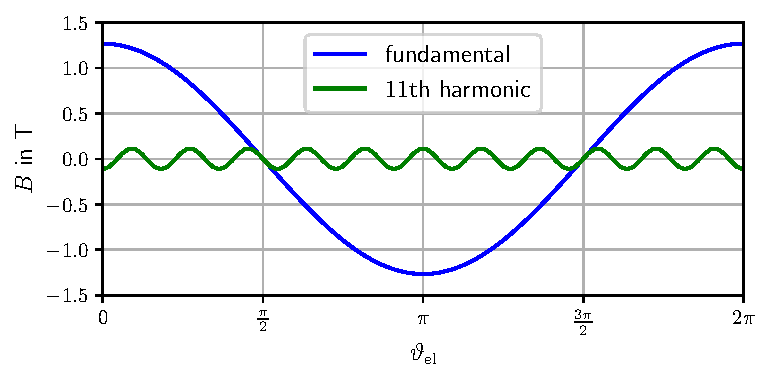
\includegraphics{FundamentalAnd11thHarmonic.pdf}
        \caption{Visualization of the flux density of the fundamental wave and the $11\textsuperscript{th}$ harmonic of phase~a.}
        \label{fig:fundamentalAnd11thHarm}
    \end{solutionfigure}    

\end{solutionblock}




%%%%%%%%%%%%%%%%%%%%%%%%%%%%%%%%%%%%%%%%%%%%%%%%%%%%%%%%%%%%%
%% Task 2 %%
%%%%%%%%%%%%%%%%%%%%%%%%%%%%%%%%%%%%%%%%%%%%%%%%%%%%%%%%%%%%%

\task{Distributed windings}
Consider a 4-pole three-phase motor with 15 stator slots. A simplified sketch of this motor with the winding scheme of phase a is shown in Fig.~\ref{fig:MMF_distributed}.

\begin{figure}[htb]
    \centering
    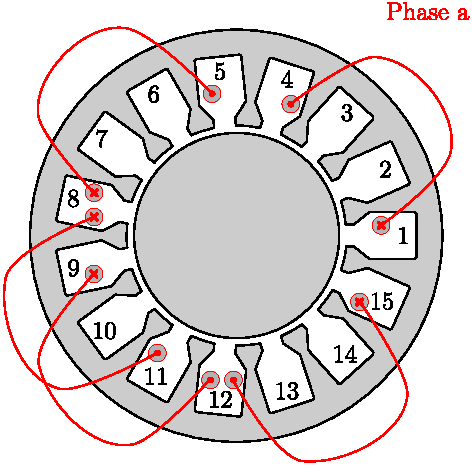
\includegraphics{MMF_distributed.pdf}
    \caption{Simplified sketch of a distributed winding scheme. Only phase a is shown.}
    \label{fig:MMF_distributed}
\end{figure}



%%%%%%%%%%%%%%%%%%%%%%%%%%%%%%%%%%%%%%%%%%%%%%%%%%%%%%%%%%%%%
\subtask{Determine the pole pitch $\tau_{\mathrm{p}}$ and the number of notches. Is it an integral-slot or a fractional-slot winding?}

\begin{solutionblock}
    The number of slots are shown in the figure, which leads to $Q$ = 15. Furthermore, the number of phases is given in the task, that is $m$ = 3.

    Hence, the pole pitch is calculated as:
    \begin{equation}
        \rho_{\mathrm{p}} = \frac{2\pi}{2p}
        = \frac{\pi}{2}.
    \end{equation}
    
    The number of notches is defined with:
    \begin{equation}
        q = \frac{Q}{2pm} = \frac{15}{2\cdot 2 \cdot 3}
        = \frac{15}{12} = \frac{5}{4}.
    \end{equation}
    Since the number of notches per pole and phase is not an integer, it is a fractional slot winding.
    The coil width $y$ is three stator slots, which leads to the angular coil width:
    \begin{equation}
        w = \frac{2\pi}{Q}m
        = \frac{2\pi}{15} \cdot 3
        = \frac{2\pi}{5}.
    \end{equation}

    Therefore, the chording factor is determined with:
    \begin{equation}
        s = \frac{w}{\tau_{\mathrm{p}}}
        = \frac{6\pi \cdot 2}{15 \pi}
        =\frac{12}{15}.
    \end{equation}

\end{solutionblock}

%%%%%%%%%%%%%%%%%%%%%%%%%%%%%%%%%%%%%%%%%%%%%%%%%%%%%%%%%%%%%
\subtask{Complete the winding scheme of the given machine in Tab.~\ref{tab:distributed_winding} for the phases b and c. Sketch the resulting winding scheme into Fig.~\ref{fig:MMF_distributed}.}

\begin{table}[ht]
    \caption{Winding scheme of the distributed winding from Fig.~\ref{fig:MMF_distributed}.}
    \centering
    \begin{tabular}{c|C{1cm}|C{1cm}|C{1cm}|C{1cm}|C{1cm}|C{1cm}}\toprule
        \multirow{2}{*}{Coil nr.} & \multicolumn{2}{c}{Phase a} & \multicolumn{2}{c}{Phase b} & \multicolumn{2}{c}{Phase c} \\
          & In  & Out   & In & Out & In & Out \\
        \midrule
        1  & 1  & 4  & & & & \\
        2  & 8  & 5  & & & & \\
        3  & 8  & 11 & & & & \\
        4  & 9  & 12 & & & & \\
        5  & 15 & 12 & & & & \\
        \bottomrule
    \end{tabular}
    \label{tab:distributed_winding}
\end{table}

\begin{solutionblock}
    In the task only phase a of the winding scheme is given. However, to complete the winding scheme, phase b must have an electrical phase shift of $\SI{120}{\degree}$ and phase c of $\SI{240}{\degree}$ respectively.
    This leads to
    \begin{equation}
        n_{\mathrm{b}} p \frac{\SI{360}{\degree}}{Q} = \SI{120}{\degree} \ \mathrm{mod} \ \SI{360}{\degree},
    \end{equation}
    where $n_{\mathrm{b}}$ is the displacement in slots. This expression is rewritten into
    \begin{equation}
        n_{\mathrm{b}} p \frac{\SI{360}{\degree}}{Q} = \SI{120}{\degree} + k \SI{360}{\degree},
        \label{eq:nb}
    \end{equation}
    and also for phase c:
    \begin{equation}
        n_{\mathrm{c}} p \frac{\SI{360}{\degree}}{Q} = \SI{240}{\degree} + k \SI{360}{\degree}.
        \label{eq:nc}
    \end{equation}
    
    Now, an integral solution must be found for \eqref{eq:nb} and \eqref{eq:nc} to determine the winding scheme.
    This is done with trial and error, the first assumption is $n_{\mathrm{b}} = 10, k = 1$, which results in
    \begin{align}
        \begin{split}
            10\cdot 2\cdot \frac{\SI{360}{\degree}}{15} &= \SI{120}{\degree}+\SI{360}{\degree}, \\
            \SI{480}{\degree} &= \SI{480}{\degree},
        \end{split}
    \end{align}
    therefore, the requirement is fulfilled. For phase c the assumption is given with $n_{\mathrm{c}} = 5, k = 1$ into \eqref{eq:nc}
    \begin{align}
        \begin{split}
            5 \cdot 2 \cdot \frac{\SI{360}{\degree}}{15} &= \SI{240}{\degree} + k \SI{360}{\degree}, \\
            \SI{240}{\degree} &= \SI{240}{\degree},
        \end{split}
    \end{align}
    which fulfills the requirement too.
    With the calculated phase shift and the knowledge of the coil width of three slots from the figure, the winding scheme is completed.
    In Tab.~\ref{tab:solution_distributedWinding} the inputs and outputs of each winding are given.
    \begin{solutiontable}
        \caption{Solution of the distributed winding scheme.}
        \centering
        \begin{tabular}{c|C{1cm}|C{1cm}|C{1cm}|C{1cm}|C{1cm}|C{1cm}}\toprule
            \multirow{2}{*}{Coil nr.} & \multicolumn{2}{c}{Phase a} & \multicolumn{2}{c}{Phase b} & \multicolumn{2}{c}{Phase c} \\
              & In  & Out   & In & Out & In & Out \\
            \midrule
            1  & 1  & 4  & 11 & 14 & 6  & 9 \\
            2  & 8  & 5  & 3  & 15 & 13 & 10 \\
            3  & 8  & 11 & 3  & 6  & 13 & 1 \\
            4  & 9  & 12 & 4  & 7  & 14 & 2 \\
            5  & 15 & 12 & 10 & 7  & 5  & 2 \\
            \bottomrule
        \end{tabular}
        \label{tab:solution_distributedWinding}
    \end{solutiontable}

    The sketch of the distributed winding scheme is visualized in Fig.~\ref{fig:solution_MMF_distributed}.
    \begin{solutionfigure}
        \centering
        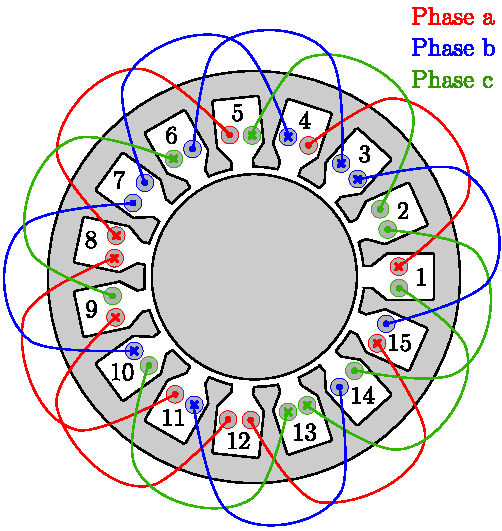
\includegraphics{solution_MMF_distributed.pdf}
        \caption{Solution of the distributed winding.}
        \label{fig:solution_MMF_distributed}
    \end{solutionfigure}

\end{solutionblock}


%%%%%%%%%%%%%%%%%%%%%%%%%%%%%%%%%%%%%%%%%%%%%%%%%%%%%%%%%%%%%
\subtask{How many layers are there in this winding scheme?}

\begin{solutionblock}
    The winding diagram has 2 winding layers, due to the two conductors per slot.
\end{solutionblock}


%%%%%%%%%%%%%%%%%%%%%%%%%%%%%%%%%%%%%%%%%%%%%%%%%%%%%%%%%%%%%
\subtask{Calculate the complex winding factors $\underline{\xi}_{\mathrm{a,}k}$ for the fundamental as well as for the $5\textsuperscript{th}$ and $7\textsuperscript{th}$ harmonic.}

\begin{solutionblock}
    The complex winding factor is defined by
    \begin{equation}
        \xi_{\mathrm{a,}k} = \frac{1}{\mathrm{j}N_{\mathrm{a}}} \sum_{i=1}^{Q} N_{\mathrm{a,}i}e^{\mathrm{j}k\vartheta_{\mathrm{el,a,}i}},
        \label{eq:complexWindingFactor}
    \end{equation}
    with
    \begin{equation}
        N_{\mathrm{a}} = \sum_{i=1}^{Q} |N_{\mathrm{a,}i} |,
    \end{equation}
    and the electrical angle:
    \begin{equation}
        \vartheta_{\mathrm{el,a,}i} = \vartheta_{\mathrm{a,}i} \cdot p.
    \end{equation}

    The mechanical angles are calculated with
    \begin{equation}
        \vartheta_{\mathrm{a,}i} = \left(i-1 \right) \frac{\SI{360}{\degree}}{Q}
        = \left(i-1 \right) \cdot \frac{\SI{360}{\degree}}{15}
        = \left(i-1 \right) \cdot \SI{24}{\degree},
    \end{equation}
    where $i$ represents the number of the stator slot.
    Therefore, the mechanical angles are given in Tab.~\ref{tab:mechanicalAngles_distributedWinding}.
    \begin{solutiontable}
        \caption{Mechanical angles of the distributed winding from Fig.~\ref{fig:MMF_distributed}.}
        \centering
        \begin{tabular}{C{3cm}|C{3cm}}\toprule
            $\vartheta_{\mathrm{a,}1} = \SI{0}{\degree}$     & $\vartheta_{\mathrm{a,}9} = \SI{192}{\degree}$ \\
            $\vartheta_{\mathrm{a,}4} = \SI{72}{\degree}$    & $\vartheta_{\mathrm{a,}11} = \SI{240}{\degree}$ \\
            $\vartheta_{\mathrm{a,}5} = \SI{96}{\degree}$    & $\vartheta_{\mathrm{a,}12} = \SI{264}{\degree}$ \\
            $\vartheta_{\mathrm{a,}8} = \SI{168}{\degree}$   & $\vartheta_{\mathrm{a,}15} = \SI{336}{\degree}$ \\
            \bottomrule
        \end{tabular}
        \label{tab:mechanicalAngles_distributedWinding}
    \end{solutiontable}

    To calculate the winding factors, the total number of turns of the respective phase $N_{\mathrm{a}}$ is determined for each stator slot. A negative sign indicates, that the winding turn is oriented towards the negative $z$-axis. When no conductor is in a slot, $N_{\mathrm{a,}i}$ = 0. The result is shown in Tab.~\ref{tab:WindingTurns_distributedWinding}.
    \begin{solutiontable}
        \caption{Winding turns of phase a of the distributed winding.}
        \centering
        \begin{tabular}{C{3cm}C{3cm}C{3cm}}\toprule
            $N_{\mathrm{a1}}$ = -1     & $N_{\mathrm{a4}}$ = 1  & $N_{\mathrm{a5}}$ = 1 \\
            $N_{\mathrm{a8}}$ = -2    & $N_{\mathrm{a9}}$ = -1   & $N_{\mathrm{a11}}$ = 1\\
            $N_{\mathrm{a12}}$ = 2  & $N_{\mathrm{a15}}$ = -1   & \\
            \bottomrule
        \end{tabular}
        \label{tab:WindingTurns_distributedWinding}
    \end{solutiontable}
    
    For the fundamental wave $k$ = 1 applies and, therefore, with \eqref{eq:complexWindingFactor}, the winding factor of the fundamental wave calculates as follows
    \begin{align}
        \begin{split}
            \underline{\xi}_{\mathrm{a,}1} = \frac{1}{10}\cdot \left[ \right. e^{j\cdot1\cdot2\cdot\SI{0}{\degree}}
            &-e^{j\cdot1\cdot2\cdot\SI{72}{\degree}}-e^{j\cdot1\cdot2\cdot\SI{92}{\degree}}+2e^{j\cdot1\cdot2\cdot\SI{168}{\degree}}+e^{j\cdot1\cdot2\cdot\SI{192}{\degree}}
            -e^{j\cdot1\cdot2\cdot\SI{240}{\degree}} \\
            & -2e^{j\cdot1\cdot2\cdot\SI{264}{\degree}}+e^{j\cdot1\cdot2\cdot\SI{336}{\degree}}
            \left. \right]
            = 0.8653 - 0.2812j,
        \end{split}
    \end{align}
    with the corresponding absolute value:
    \begin{equation}
        |\xi_{\mathrm{a,}1}| = 0.9099.
    \end{equation}

    For the $5\textsuperscript{th}$ harmonic is $k$ = 5, which results in
    \begin{align}
        \begin{split}
            \underline{\xi}_{\mathrm{a,}5} = \frac{1}{10}\cdot \left[ \right. e^{j\cdot5\cdot2\cdot\SI{0}{\degree}}
            &-e^{j\cdot5\cdot2\cdot\SI{72}{\degree}}-e^{j\cdot5\cdot2\cdot\SI{92}{\degree}}+2e^{j\cdot5\cdot2\cdot\SI{168}{\degree}}+e^{j\cdot5\cdot2\cdot\SI{192}{\degree}}
            -e^{j\cdot5\cdot2\cdot\SI{240}{\degree}} \\
            & -2e^{j\cdot5\cdot2\cdot\SI{264}{\degree}}+e^{j\cdot5\cdot2\cdot\SI{336}{\degree}}
            \left. \right]
            = 0,
        \end{split}
    \end{align}
    with the corresponding absolute value:
    \begin{equation}
        |\xi_{\mathrm{a,}5}| = 0.
    \end{equation}

    The complex winding factor for the $7\textsuperscript{th}$ harmonic results by
    \begin{align}
        \begin{split}
            \underline{\xi}_{\mathrm{a,}7} = \frac{1}{10}\cdot \left[ \right. e^{j\cdot7\cdot2\cdot\SI{0}{\degree}}
            &-e^{j\cdot7\cdot2\cdot\SI{72}{\degree}}-e^{j\cdot7\cdot2\cdot\SI{92}{\degree}}+2e^{j\cdot7\cdot2\cdot\SI{168}{\degree}}+e^{j\cdot7\cdot2\cdot\SI{192}{\degree}}
            -e^{j\cdot7\cdot2\cdot\SI{240}{\degree}} \\
            & -2e^{j\cdot7\cdot2\cdot\SI{264}{\degree}}+e^{j\cdot7\cdot2\cdot\SI{336}{\degree}}
            \left. \right]
            = -0.0516- 0.0711j,
        \end{split}
    \end{align}
    with the corresponding absolute value:
    \begin{equation}
        |\xi_{\mathrm{a,}7}| = 0.087.
    \end{equation}


\end{solutionblock}


%%%%%%%%%%%%%%%%%%%%%%%%%%%%%%%%%%%%%%%%%%%%%%%%%%%%%%%%%%%%%
\subtask{Assume a block-shaped distribution of the flux density with a maximal value of $\hat{B} = \SI{1}{\tesla}$ and a number of winding turns $N'_{\mathrm{a}}$ = 30 (i.e., there are more turns per coil as indicated within Fig.~\ref{fig:MMF_distributed}). The axial length of the machine is $l=\SI{0.35}{\metre}$ and the diameter is $d_{\mathrm{s}} = \SI{0.10}{\metre}$. The machine rotates with a mechanical speed of $n=\SI{250}{\per \minute}$. Calculate the induced voltage of phase a for the fundamental wave as well as of the $5\textsuperscript{th}$ and $7\textsuperscript{th}$ harmonics.}

\begin{solutionblock}
    The Fourier coefficient of the flux density is given with
    \begin{equation}
        B(\vartheta_{\mathrm{el}},t) = \frac{6}{\pi p} \hat{B} \sum_{k}^{\infty} \frac{1}{k} \sin\left(\frac{k\pi}{2} \right) \cos(\omega t - k \vartheta_{\mathrm{el}}),
    \end{equation}
    and for the fundamental wave:
    \begin{equation}
        B^{(1)}(\vartheta_{\mathrm{el}},t) = \frac{6}{\pi p} \hat{B} \sin\left(\frac{\pi}{2}\right) \cos(\omega t - \vartheta_{\mathrm{el}}).
    \end{equation}

    The flux linkage of phase a is calculated as
    \begin{equation}
        \phi_{\mathrm{a,}k}(t) = l \frac{d_{\mathrm{s}}}{2} |\xi_{\mathrm{a},k}| \int_{-\frac{\pi}{2}}^{\frac{\pi}{2}} B(\vartheta_{\mathrm{el}},t) \mathrm{d}\vartheta_{\mathrm{el}},
        \label{eq:phi_a_k}
    \end{equation}
    with the complex winding factor to cover the winding distribution inside the stator.
    Hence, the fundamental wave calculates as follows:
    \begin{align}
        \begin{split}
            \phi_{\mathrm{a,}1}(t) &= l \frac{d_{\mathrm{s}}}{2} |\xi_{\mathrm{a},1}|
            \frac{6}{\pi p} \hat{B} \sin\left(\frac{\pi}{2}\right) \int_{-\frac{\pi}{2}}^{\frac{\pi}{2}} \cos(\omega t - \vartheta_{\mathrm{el}}) \mathrm{d}\vartheta_{\mathrm{el}} \\
            &= l d_{\mathrm{s}} |\xi_{\mathrm{a},1}|
            \frac{3}{\pi p} \hat{B}
            \int_{-\frac{\pi}{2}}^{\frac{\pi}{2}}\cos(\omega t) \cos(\vartheta_{\mathrm{el}}) + \sin(\omega t) \sin(\vartheta_{\mathrm{el}}) \mathrm{d}\vartheta_{\mathrm{el}} \\
            &= l d_{\mathrm{s}} |\xi_{\mathrm{a},1}|
            \frac{3}{\pi p} \hat{B}
            \left[\cos(\omega t) \int_{-\frac{\pi}{2}}^{\frac{\pi}{2}} \cos(\vartheta_{\mathrm{el}}) \mathrm{d}\vartheta_{\mathrm{el}} + \sin(\omega t) \int_{-\frac{\pi}{2}}^{\frac{\pi}{2}} \sin(\vartheta_{\mathrm{el}}) \mathrm{d} \vartheta_{\mathrm{el}} \right] \\
            &= l d_{\mathrm{s}} |\xi_{\mathrm{a},1}|
            \frac{3}{\pi p} \hat{B}
            \left[\cos(\omega t) \left[\sin(\vartheta_{\mathrm{el}}) \right]_{-\frac{\pi}{2}}^{\frac{\pi}{2}} + \sin(\omega t) \left[-\cos(\vartheta_{\mathrm{el}}) \right]_{-\frac{\pi}{2}}^{\frac{\pi}{2}} \right] \\
            &= l d_{\mathrm{s}} |\xi_{\mathrm{a},1}|
            \frac{3}{\pi p} \hat{B} \left[ 2 \cos(\omega t)\right] \\
            &= l d_{\mathrm{s}} |\xi_{\mathrm{a},1}|
            \frac{6}{\pi p} \hat{B} \cos(\omega t). \\
        \end{split}
    \end{align}

   Taking into account also the number of winding turns $N_{\mathrm{a}}$, the flux linkage of phase a is given with 
    \begin{equation}
        \psi_{\mathrm{a,}k}(t) = N_{\mathrm{a}}' \phi_{\mathrm{a,}k}(t),
        \label{eq:psi_a_k}
    \end{equation}
    which results for the fundamental wave into:
    \begin{align}
        \begin{split}
            \psi_{\mathrm{a,}1}(t) &= N_{\mathrm{a}}' \phi_{\mathrm{a,}k}(t) 
            = N_{\mathrm{a}}' l d_{\mathrm{s}} |\xi_{\mathrm{a},1}| \frac{6}{\pi p} \hat{B} \cos(\omega t) \\
            &= 30 \cdot \SI{0.35}{\metre} \cdot \SI{0.10}{\metre} \cdot \frac{6}{2\pi} \cdot \SI{1}{\tesla} \cos(\omega t) \cdot 0.9099 \\
            &= \SI{0.9123}{\volt\second} \cdot \cos(\omega t).
        \end{split}
    \end{align}

    The equation for the induced voltage of the fundamental wave is given with:
    \begin{align}
        \begin{split}
            u_{\mathrm{ind,a,}1}(t) &= -\frac{\mathrm{d}}{\mathrm{d}t}\psi_{\mathrm{a,}1} \\
            &= -\frac{\mathrm{d}}{\mathrm{d}t} \SI{0.9123}{\volt\second} \cdot \cos(\omega t) \\
            &= \SI{0.9123}{\volt\second} \cdot \sin(\omega t) \omega \\
            &= \SI{0.9123}{\volt\second} \cdot \sin(\omega t) \cdot 2\pi \cdot 2 \cdot \SI{\frac{250}{60}}{\per\second} \\
            &= \SI{47.78}{\volt} \cdot \sin(\omega t).
        \end{split}
    \end{align}

    The flux linkage of the $5\textsuperscript{th}$ harmonic is determined with \eqref{eq:phi_a_k}, which results into
    \begin{equation}
        \phi_{\mathrm{a},5} = 0,
    \end{equation}
    due to $|\xi_{\mathrm{a},5}|$ = 0. Therefore, the induced voltage results by:
    \begin{equation}
        u_{\mathrm{ind,a,}5}  = 0.
    \end{equation}

    With \eqref{eq:phi_a_k} the flux linkage for the $7\textsuperscript{th}$ harmonic is calculated by:
    \begin{align}
        \begin{split}
            \phi_{\mathrm{a,}7}(t) &= l \frac{d_{\mathrm{s}}}{2} |\xi_{\mathrm{a},7}|
            \frac{6}{\pi p} \hat{B}\frac{1}{7} \sin\left(\frac{7\pi}{2}\right) \int_{-\frac{\pi}{2}}^{\frac{\pi}{2}} \cos(\omega t - 7\vartheta_{\mathrm{el}}) \mathrm{d}\vartheta_{\mathrm{el}} \\
            &  \vdots \\
            &= l \frac{d_{\mathrm{s}}}{2} |\xi_{\mathrm{a},7}|
            \frac{6}{\pi p} \hat{B} \frac{1}{7} \cos(\omega t).
        \end{split}
    \end{align}

    The resulting flux linkage is calculated by taking into account the number of winding turns as
    \begin{align}
        \begin{split}
            \psi_{\mathrm{a,}7} &= N_{\mathrm{a}}' \phi_{\mathrm{a,}7}(t) 
            = N_{\mathrm{a}}' l \frac{d_{\mathrm{s}}}{2} |\xi_{\mathrm{a},7}| \frac{6}{\pi p} \hat{B} \frac{1}{7} \cos(\omega t) \\
            &= 30 \cdot \SI{0.35}{\metre} \cdot \SI{\frac{10}{2}}{\metre} \cdot \frac{6}{2\pi} \cdot \SI{1}{\tesla} \cdot \frac{1}{7} \cdot \cos(\omega t) \cdot 0.087 \\
            &= \SI{0.0126}{\volt\second} \cdot \cos(\omega t),
        \end{split}
    \end{align}
    therefore, the induced voltage is given with:
    \begin{align}
        \begin{split}
            u_{\mathrm{ind,a,}7}(t) &= -\frac{\mathrm{d}}{\mathrm{d}t}\psi_{\mathrm{a,}7} \\
            &= \SI{0.0126}{\volt\second} \cdot \sin(\omega t) \omega \\
            &= \SI{0.0126}{\volt\second} \cdot \sin(\omega t) \cdot \SI{2\pi\cdot 2\cdot \frac{250}{60}}{\per\second} \\
            &= \SI{0.66}{\volt} \cdot \sin(\omega t).
        \end{split}
    \end{align}
    
\end{solutionblock}



%%%%%%%%%%%%%%%%%%%%%%%%%%%%%%%%%%%%%%%%%%%%%%%%%%%%%%%%%%%%%
\subtask{Write a Python script to calcualte the complex winding factor $\underline{\xi}_{\mathrm{a,}k}$ up to various harmonics.}

\begin{solutionblock}
    The Python script is separately available, therefore, only the solution is presented in Tab~\ref{tab:complexWindingFactor_python}.
    \begin{solutiontable}
        \caption{Complex winding factor $\underline{\xi}_{\mathrm{a,}k}$ up to the $12\textsuperscript{th}$ harmonic order.}
        \centering
        \begin{tabular}{R{5cm}R{5cm}R{5cm}}\toprule
              $\underline{\xi}_{\mathrm{a,}1}$ = 0.8653-0.2812j
            & $\underline{\xi}_{\mathrm{a,}2}$ = 0.0353+0.0486j
            & $\underline{\xi}_{\mathrm{a,}3}$ = 0.2236-0.3078j \\
              $\underline{\xi}_{\mathrm{a,}4}$ = -0.099-0.0322j
            & $\underline{\xi}_{\mathrm{a,}5}$ = 0
            & $\underline{\xi}_{\mathrm{a,}6}$ = -0.2236+0.0727j \\
              $\underline{\xi}_{\mathrm{a,}7}$ = -0.0516-0.0711j
            & $\underline{\xi}_{\mathrm{a,}8}$ = -0.0516+0.0711j
            & $\underline{\xi}_{\mathrm{a,}9}$ = -0.2236-0.0727j \\
              $\underline{\xi}_{\mathrm{a,}10}$ = 0
            & $\underline{\xi}_{\mathrm{a,}11}$ = -0.099+0.0322j
            & $\underline{\xi}_{\mathrm{a,}12}$ = 0.2236+0.3078j \\
            \bottomrule
        \end{tabular}
        \label{tab:complexWindingFactor_python}
    \end{solutiontable}
\end{solutionblock}




%%%%%%%%%%%%%%%%%%%%%%%%%%%%%%%%%%%%%%%%%%%%%%%%%%%%%%%%%%%%%
%% Task 3 %%
%%%%%%%%%%%%%%%%%%%%%%%%%%%%%%%%%%%%%%%%%%%%%%%%%%%%%%%%%%%%%

\task{Concentrated windings}
Consider the shown 10-pole 3-phase motor with 12 stator slots in Fig.~\ref{fig:MMF_concentrated}. The winding scheme of phase a is shown in the figure.

\begin{figure}[htb]
    \centering
    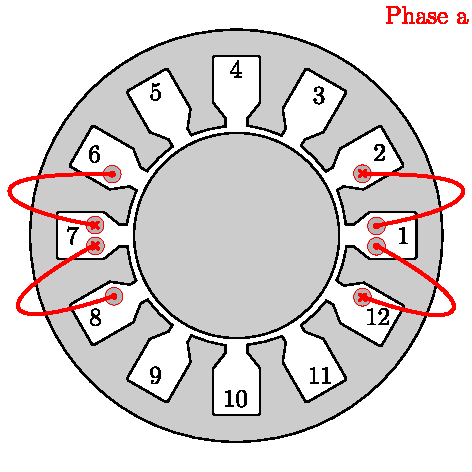
\includegraphics{MMF_concentrated.pdf}
    %\captionsetup{labelfont={color=blue},textfont={color=blue}}
    \caption{Simplified sketch of a concentrated winding. Only phase a is shown.}
    \label{fig:MMF_concentrated}
\end{figure}

%%%%%%%%%%%%%%%%%%%%%%%%%%%%%%%%%%%%%%%%%%%%%%%%%%%%%%%%%%%%%
\subtask{Determine the pole pitch and und the number of notches. Is it an integral-slot or a fractional-slot winding?}

\begin{solutionblock}
    The number of slots is determined by counting the slots in the given figure of the machine.
    Hence, the number of slots is $Q$ = 12. The number of phases is given in the task, which is $m$=3.
    Therefore, the pole pitch calculates as:
    \begin{equation}
        \rho_{\mathrm{p}} = \frac{2\pi}{2p}
        = \frac{\pi}{5}.
    \end{equation}

    The number of notches is determined with:
    \begin{equation}
        q = \frac{Q}{2pm}
        = \frac{12}{2 \cdot 5 \cdot 3}
        = \frac{2}{5}.
    \end{equation}
    Since the number of notches per pole and phase is not an integer, it is a fractional slot winding.
    The coil width $y$ is one stator slot, as it is shown in the figure. This results in the angular coil width: 
    \begin{equation}
        w = \frac{2\pi}{Q}
        = \frac{2\pi}{12}
        = \frac{\pi}{6}.
    \end{equation}

    Hence, the chording factor is calculated by:
    \begin{equation}
        s = \frac{w}{\tau_{\mathrm{p}}}
        = \frac{\pi \cdot 5}{6\pi}
        = \frac{5}{6}.
    \end{equation}

\end{solutionblock}

%%%%%%%%%%%%%%%%%%%%%%%%%%%%%%%%%%%%%%%%%%%%%%%%%%%%%%%%%%%%%
\subtask{Complete Tab.~\ref{tab:concentrated_winding} with the winding scheme for phases b and c. Sketch the resulting winding scheme in Fig.~\ref{fig:MMF_concentrated}.}

\begin{table}[ht]
    \caption{Winding scheme of a concentrated winding from Fig.~\ref{fig:MMF_concentrated}.}
    \centering
    \begin{tabular}{c|C{1cm}|C{1cm}|C{1cm}|C{1cm}|C{1cm}|C{1cm}}\toprule
        \multirow{2}{*}{Coil nr.} & \multicolumn{2}{c}{Phase a} & \multicolumn{2}{c}{Phase b} & \multicolumn{2}{c}{Phase c} \\
          & In  & Out   & In & Out & In & Out \\
        \midrule
        1  & 1  & 2  & & & & \\
        2  & 1  & 12  & & & & \\
        3  & 7  & 6  & & & & \\
        4  & 7  & 8  & & & & \\
        \bottomrule
    \end{tabular}
    \label{tab:concentrated_winding}
\end{table}


\begin{solutionblock}
    In the task only phase a of the winding scheme is given. However, to complete the winding scheme, phase b must have an electrical phase shift of $\SI{120}{\degree}$ and phase c of $\SI{240}{\degree}$ respectively.
    This leads to
    \begin{equation}
        n_{\mathrm{b}} p \frac{\SI{360}{\degree}}{Q} = \SI{120}{\degree} \ \mathrm{mod} \ \SI{360}{\degree},
    \end{equation}
    where $n_{\mathrm{b}}$ is the displacement in slots. This expression is rewritten into
    \begin{equation}
        n_{\mathrm{b}} p \frac{\SI{360}{\degree}}{Q} = \SI{120}{\degree} + k \SI{360}{\degree},
        \label{eq:nb_concentrated}
    \end{equation}
    and also for phase c:
    \begin{equation}
        n_{\mathrm{c}} p \frac{\SI{360}{\degree}}{Q} = \SI{240}{\degree} + k \SI{360}{\degree}.
        \label{eq:nc_concentrated}
    \end{equation}
    
    Now, an integral solution must be found for \eqref{eq:nb_concentrated} and \eqref{eq:nc_concentrated} to determine the winding scheme.
    This is done with trial and error, the first assumption is $n_{\mathrm{b}} = 8, k = 3$, which results in
    \begin{align}
        \begin{split}
            8\cdot 5\cdot \frac{\SI{360}{\degree}}{12} &= \SI{120}{\degree}+3 \cdot \SI{360}{\degree}, \\
            \SI{1200}{\degree} &= \SI{1200}{\degree},
        \end{split}
    \end{align}
    therefore, the requirement is fulfilled. For phase c the assumption is given with $n_{\mathrm{c}} = 4, k = 1$ into \eqref{eq:nc_concentrated} leads to
    \begin{align}
        \begin{split}
            4 \cdot 5 \cdot \frac{\SI{360}{\degree}}{12} &= \SI{240}{\degree} + k \SI{360}{\degree}, \\
            \SI{600}{\degree} &= \SI{600}{\degree},
        \end{split}
    \end{align}
    which fulfills the requirement too.

    With the coil width of one slot, the resulting winding is determined. The solution of this winding scheme is shown in Tab.~\ref{tab:solution_concentratedWinding}.
    \begin{solutiontable}
        \caption{Solution of the winding scheme of a concentrated winding.}
        \centering
        \begin{tabular}{c|C{1cm}|C{1cm}|C{1cm}|C{1cm}|C{1cm}|C{1cm}}\toprule
            \multirow{2}{*}{Coil nr.} & \multicolumn{2}{c}{Phase a} & \multicolumn{2}{c}{Phase b} & \multicolumn{2}{c}{Phase c} \\
              & In  & Out   & In & Out & In & Out \\
            \midrule
            1  & 1  & 2  & 3 & 2 & 4 & 5 \\
            2  & 1 & 12  & 3 & 4 & 6 & 5 \\
            3  & 7  & 6  & 8 & 9 & 11 & 10 \\
            4  & 7  & 8  & 10 & 9 & 11 & 12\\
            \bottomrule
        \end{tabular}
        \label{tab:solution_concentratedWinding}
    \end{solutiontable}
    

    The completed winding scheme is visualized in Fig.\ref{fig:solution_MMF_concentrated}.
    \begin{solutionfigure}
        \centering
        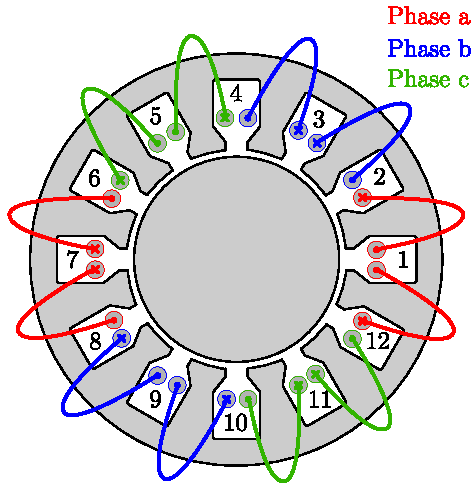
\includegraphics{solution_MMF_concentrated.pdf}
        \captionsetup{labelfont={color=blue},textfont={color=blue}}
        \caption{Solution of the concentrated winding scheme.}
        \label{fig:solution_MMF_concentrated}
    \end{solutionfigure}
\end{solutionblock}



%%%%%%%%%%%%%%%%%%%%%%%%%%%%%%%%%%%%%%%%%%%%%%%%%%%%%%%%%%%%%
\subtask{How many layers are in this winding scheme?}

\begin{solutionblock}
    There are two layers per slot, therefore, it is a two layer winding scheme.
\end{solutionblock}

%%%%%%%%%%%%%%%%%%%%%%%%%%%%%%%%%%%%%%%%%%%%%%%%%%%%%%%%%%%%%
\subtask{Calculate the complex winding factors $\underline{\xi}_{\mathrm{a,}k}$ for the fundamental as well as for the $5\textsuperscript{th}$ and $7\textsuperscript{th}$ harmonic.}

\begin{solutionblock}
    The complex winding factor is defined by
    \begin{equation}
        \underline{\xi}_{\mathrm{a,}k} = \frac{1}{\mathrm{j}N_{\mathrm{a}}} \sum_{i=1}^{Q} N_{\mathrm{a,}i}e^{\mathrm{j}k\vartheta_{\mathrm{el,a,}i}},
        \label{eq:complexWindingFactor_concentratedWinding}
    \end{equation}
    with
    \begin{equation}
        N_{\mathrm{a}} = \sum_{i=1}^{Q} |N_{\mathrm{a,}i} |,
    \end{equation}
    and the electrical angle:
    \begin{equation}
        \vartheta_{\mathrm{el,a,}i} = \vartheta_{\mathrm{a,}i} \cdot p.
    \end{equation}
    
    Hence, the mechanical angles are calculated as follows
    \begin{equation}
        \vartheta_{\mathrm{a,}i} = \left(i-1 \right) \frac{\SI{360}{\degree}}{Q}
        = \left(i-1 \right) \cdot \frac{\SI{360}{\degree}}{12}
        = \left(i-1 \right)\cdot \SI{30}{\degree},
    \end{equation}
    where $i$ represents the number of the stator slot.
    Therefore, the mechanical angles are given in Tab.~\ref{tab:mechanicalAngles_concentratedWinding}.
    \begin{solutiontable}
        \caption{Mechanical angles of the concentrated winding from Fig.~\ref{fig:MMF_concentrated}.}
        \centering
        \begin{tabular}{C{3cm}|C{3cm}}\toprule
            $\vartheta_{\mathrm{a,}1} = \SI{0}{\degree}$     & $\vartheta_{\mathrm{a,}9} = \SI{180}{\degree}$ \\
            $\vartheta_{\mathrm{a,}4} = \SI{30}{\degree}$    & $\vartheta_{\mathrm{a,}11} = \SI{210}{\degree}$ \\
            $\vartheta_{\mathrm{a,}5} = \SI{150}{\degree}$    & $\vartheta_{\mathrm{a,}12} = \SI{330}{\degree}$ \\
            \bottomrule
        \end{tabular}
        \label{tab:mechanicalAngles_concentratedWinding}
    \end{solutiontable}

    To calculate the winding factors, the total number of turns of the respective phase $N_{\mathrm{a}}$ is determined for each stator slot. A negative sign indicates, that the winding turn is oriented towards the negative $z$-axis. When no conductor is in a slot, $N_{\mathrm{a,}i}$ = 0. The result is shown in Tab.~\ref{tab:WindingTurns_concentratedWinding}.
    \begin{solutiontable}
        \caption{Winding turns of phase a of the concentrated winding rom Fig.~\ref{fig:MMF_concentrated}.}
        \centering
        \begin{tabular}{C{3cm}C{3cm}C{3cm}}\toprule
            $N_{\mathrm{a1}}$ = 2     & $N_{\mathrm{a2}}$ = -1  & $N_{\mathrm{a6}}$ = 1 \\
            $N_{\mathrm{a7}}$ = -2    & $N_{\mathrm{a8}}$ = 1   & $N_{\mathrm{a12}}$ = -1\\
            \bottomrule
        \end{tabular}
        \label{tab:WindingTurns_concentratedWinding}
    \end{solutiontable}
    
    For the fundamental wave, is $k$ = 1 and, therefore, with \eqref{eq:complexWindingFactor_concentratedWinding}, the winding factor of the fundamental wave calculates as follows:
    \begin{equation}
        \underline{\xi}_{\mathrm{a,}1} = \frac{1}{8}\cdot \left[ \right. -2e^{j\cdot1\cdot5\cdot\SI{0}{\degree}}
        +e^{j\cdot1\cdot5\cdot\SI{30}{\degree}}-e^{j\cdot1\cdot5\cdot\SI{150}{\degree}}+2e^{j\cdot1\cdot5\cdot\SI{180}{\degree}}-e^{j\cdot1\cdot5\cdot\SI{210}{\degree}}
        +e^{j\cdot1\cdot5\cdot\SI{330}{\degree}}
        \left. \right]
        = -0.9330,
    \end{equation}
    with the absolute value:
    \begin{equation}
        |\xi_{\mathrm{a,}1}| = 0.9330.
    \end{equation}

    For the $5\textsuperscript{th}$ harmonic is $k$ = 5, which results in
    \begin{equation}
        \underline{\xi}_{\mathrm{a,}5} = \frac{1}{8}\cdot \left[ \right. -2e^{j\cdot5\cdot5\cdot\SI{0}{\degree}}
        +e^{j\cdot5\cdot5\cdot\SI{30}{\degree}}-e^{j\cdot5\cdot5\cdot\SI{150}{\degree}}+2e^{j\cdot5\cdot5\cdot\SI{180}{\degree}}-e^{j\cdot5\cdot5\cdot\SI{210}{\degree}}
        +e^{j\cdot5\cdot5\cdot\SI{330}{\degree}}
        \left. \right]
        = -0.067,
    \end{equation}
    with the absolute value:
    \begin{equation}
        |\xi_{\mathrm{a,}5}| = 0.067.
    \end{equation}

    Finally, the complex winding factor for the $7\textsuperscript{th}$ harmonic is defined as
    \begin{equation}
        |\xi_{\mathrm{a,}7}| = \frac{1}{8}\cdot \left[ \right. -2e^{j\cdot7\cdot5\cdot\SI{0}{\degree}}
        +e^{j\cdot7\cdot5\cdot\SI{30}{\degree}}-e^{j\cdot7\cdot5\cdot\SI{150}{\degree}}+2e^{j\cdot7\cdot5\cdot\SI{180}{\degree}}-e^{j\cdot7\cdot5\cdot\SI{210}{\degree}}
        +e^{j\cdot7\cdot5\cdot\SI{330}{\degree}}
        \left. \right]
        = -0.067,
    \end{equation}
    and, therefore, the absolute value results in:
    \begin{equation}
        |\xi_{\mathrm{a,}7}| = 0.067.
    \end{equation}

    As can be seen from the calculations of the complex winding factors $|\xi_{\mathrm{a,}1}|,|\xi_{\mathrm{a,}5}|$ and $|\xi_{\mathrm{a,}7}|$, these only have a real part.

\end{solutionblock}


%%%%%%%%%%%%%%%%%%%%%%%%%%%%%%%%%%%%%%%%%%%%%%%%%%%%%%%%%%%%%
\subtask{Assume a block-shaped distribution of the flux density with a maximal value of $\hat{B} = \SI{1}{\tesla}$ and a number of winding turns $N'_{\mathrm{a}}$ = 137. The axial length of the machine is $l=\SI{0.70}{\metre}$ and the diameter is $d = \SI{0.45}{\metre}$. The machine rotates with a mechanical speed of $n=\SI{50}{\per \minute}$. Calculate the induced voltage of phase a for the fundamental wave. What are the $5\textsuperscript{th}$ and $7\textsuperscript{th}$ harmonics of the induced voltage in phase a?}

\begin{solutionblock}
    The Fourier coefficient of the flux density is given with
    \begin{equation}
        B(\vartheta_{\mathrm{el}},t) = \frac{6}{\pi p} \hat{B} \sum_{k}^{\infty} \frac{1}{k} \sin\left(\frac{k\pi}{2} \right) \cos(\omega t - k \vartheta_{\mathrm{el}}),
    \end{equation}
    and for the fundamental wave:
    \begin{equation}
        B^{(1)}(\vartheta_{\mathrm{el}},t) = \frac{6}{\pi p} \hat{B} \sin\left(\frac{\pi}{2}\right) \cos(\omega t - \vartheta_{\mathrm{el}}).
    \end{equation}

    The flux linkage of phase a is calculated as
    \begin{equation}
        \phi_{\mathrm{a,}k}(t) = l \frac{d_{\mathrm{s}}}{2} |\xi_{\mathrm{a},k}| \int_{-\frac{\pi}{2}}^{\frac{\pi}{2}} B(\vartheta_{\mathrm{el}},t) \mathrm{d}\vartheta_{\mathrm{el}},
        \label{eq:phi_a_k_concentrated}
    \end{equation}
    with the complex winding factor to cover the winding distribution inside the stator.
    Hence, the fundamental wave calculates as follows:
    \begin{align}
        \begin{split}
            \phi_{\mathrm{a,}1}(t) &= l \frac{d_{\mathrm{s}}}{2} |\xi_{\mathrm{a},1}|
            \frac{6}{\pi p} \hat{B} \sin\left(\frac{\pi}{2}\right) \int_{-\frac{\pi}{2}}^{\frac{\pi}{2}} \cos(\omega t - \vartheta_{\mathrm{el}}) \mathrm{d}\vartheta_{\mathrm{el}} \\
            &= l d_{\mathrm{s}} |\xi_{\mathrm{a},1}|
            \frac{3}{\pi p} \hat{B}
            \int_{-\frac{\pi}{2}}^{\frac{\pi}{2}}\cos(\omega t) \cos(\vartheta_{\mathrm{el}}) + \sin(\omega t) \sin(\vartheta_{\mathrm{el}}) \mathrm{d}\vartheta_{\mathrm{el}} \\
            &= l d_{\mathrm{s}} |\xi_{\mathrm{a},1}|
            \frac{3}{\pi p} \hat{B}
            \left[\cos(\omega t) \int_{-\frac{\pi}{2}}^{\frac{\pi}{2}} \cos(\vartheta_{\mathrm{el}}) \mathrm{d}\vartheta_{\mathrm{el}} + \sin(\omega t) \int_{-\frac{\pi}{2}}^{\frac{\pi}{2}} \sin(\vartheta_{\mathrm{el}}) \mathrm{d} \vartheta_{\mathrm{el}} \right] \\
            &= l d_{\mathrm{s}} |\xi_{\mathrm{a},1}|
            \frac{3}{\pi p} \hat{B}
            \left[\cos(\omega t) \left[\sin(\vartheta_{\mathrm{el}}) \right]_{-\frac{\pi}{2}}^{\frac{\pi}{2}} + \sin(\omega t) \left[-\cos(\vartheta_{\mathrm{el}}) \right]_{-\frac{\pi}{2}}^{\frac{\pi}{2}} \right] \\
            &= l d_{\mathrm{s}} |\xi_{\mathrm{a},1}|
            \frac{3}{\pi p} \hat{B} \left[ 2 \cos(\omega t)\right] \\
            &= l d_{\mathrm{s}} |\xi_{\mathrm{a},1}|
            \frac{6}{\pi p} \hat{B} \cos(\omega t). \\
        \end{split}
    \end{align}

   Taking into account also the number of winding turns $N_{\mathrm{a}}$, the flux linkage of phase a is given with 
    \begin{equation}
        \psi_{\mathrm{a,}k}(t) = N_{\mathrm{a}}' \phi_{\mathrm{a,}k}(t),
        \label{eq:psi_a_k_concentrated}
    \end{equation}
    which results for the fundamental wave into:
    \begin{align}
        \begin{split}
            \psi_{\mathrm{a,}1}(t) &= N_{\mathrm{a}}' \phi_{\mathrm{a,}k}(t) 
            = N_{\mathrm{a}}' l d_{\mathrm{s}} |\xi_{\mathrm{a},1}| \frac{6}{\pi p} \hat{B} \cos(\omega t) \\
            &= 137 \cdot \SI{0.7}{\metre} \cdot \SI{0.45}{\metre} \cdot \frac{6}{5\pi} \cdot \SI{1}{\tesla} \cos(\omega t) \cdot 0.9330 \\
            &= \SI{15.38}{\volt\second} \cdot \cos(\omega t).
        \end{split}
    \end{align}

    The equation for the induced voltage of the fundamental wave is given with:
    \begin{align}
        \begin{split}
            u_{\mathrm{ind,a,}1}(t) &= -\frac{\mathrm{d}}{\mathrm{d}t}\psi_{\mathrm{a,}1} \\
            &= -\frac{\mathrm{d}}{\mathrm{d}t} \SI{15.38}{\volt\second} \cdot \cos(\omega t) \\
            &= \SI{15.38}{\volt\second} \cdot \sin(\omega t) \omega \\
            &= \SI{15.38}{\volt\second} \cdot \sin(\omega t) \cdot 2\pi \cdot 5 \cdot \SI{\frac{50}{60}}{\per\second} \\
            &= \SI{402.6}{\volt} \cdot \sin(\omega t).
        \end{split}
    \end{align}

    The flux linkage of the $5\textsuperscript{th}$ harmonic is determined with \eqref{eq:phi_a_k_concentrated}, which results into:
    \begin{align}
        \begin{split}
            \phi_{\mathrm{a,}5}(t) &= l \frac{d_{\mathrm{s}}}{2} |\xi_{\mathrm{a},5}|
            \frac{6}{\pi p} \hat{B}\frac{1}{5} \sin\left(\frac{5\pi}{2}\right) \int_{-\frac{\pi}{2}}^{\frac{\pi}{2}} \cos(\omega t - 5\vartheta_{\mathrm{el}}) \mathrm{d}\vartheta_{\mathrm{el}} \\
            &  \vdots \\
            &= l \frac{d_{\mathrm{s}}}{2} |\xi_{\mathrm{a},5}|
            \frac{6}{\pi p} \hat{B} \frac{1}{5} \cos(\omega t).
        \end{split}
    \end{align}
    The resulting flux linkage is calculated by taking into account the number of winding turns as
    \begin{align}
        \begin{split}
            \psi_{\mathrm{a,}5} &= N_{\mathrm{a}}' \phi_{\mathrm{a,}5}(t) 
            = N_{\mathrm{a}}' l \frac{d_{\mathrm{s}}}{2} |\xi_{\mathrm{a},5}| \frac{6}{\pi p} \hat{B} \frac{1}{5} \cos(\omega t) \\
            &= 137 \cdot \SI{0.7}{\metre} \cdot \SI{\frac{0.45}{2}}{\metre} \cdot \frac{6}{5\pi} \cdot \SI{1}{\tesla} \cdot \frac{1}{5} \cdot \cos(\omega t) \cdot 0.0067 \\
            &= \SI{0.2208}{\volt\second} \cdot \cos(\omega t),
        \end{split}
    \end{align}
    therefore, the induced voltage is given with:
    \begin{align}
        \begin{split}
            u_{\mathrm{ind,a,}5}(t) &= -\frac{\mathrm{d}}{\mathrm{d}t}\psi_{\mathrm{a,}5} \\
            &= \SI{0.2208}{\volt\second} \cdot \sin(\omega t) \omega \\
            &= \SI{0.2208}{\volt\second} \cdot \SI{2\pi\cdot 5\cdot \frac{50}{60}}{\per\second} \\
            &= \SI{5.78}{\volt} \cdot \sin(\omega t).
        \end{split}
    \end{align}
    

    With \eqref{eq:phi_a_k} the flux linkage for the $7\textsuperscript{th}$ harmonic is calculated by:
    \begin{align}
        \begin{split}
            \phi_{\mathrm{a,}7}(t) &= l \frac{d_{\mathrm{s}}}{2} |\xi_{\mathrm{a},7}|
            \frac{6}{\pi p} \hat{B}\frac{1}{7} \sin\left(\frac{7\pi}{2}\right) \int_{-\frac{\pi}{2}}^{\frac{\pi}{2}} \cos(\omega t - 7\vartheta_{\mathrm{el}}) \mathrm{d}\vartheta_{\mathrm{el}} \\
            &  \vdots \\
            &= l \frac{d_{\mathrm{s}}}{2} |\xi_{\mathrm{a},7}|
            \frac{6}{\pi p} \hat{B} \frac{1}{7} \cos(\omega t).
        \end{split}
    \end{align}

    The resulting flux linkage is calculated by taking into account the number of winding turns as
    \begin{align}
        \begin{split}
            \psi_{\mathrm{a,}7} &= N_{\mathrm{a}}' \phi_{\mathrm{a,}7}(t) 
            = N_{\mathrm{a}}' l \frac{d_{\mathrm{s}}}{2} |\xi_{\mathrm{a},7}| \frac{6}{\pi p} \hat{B} \frac{1}{7} \cos(\omega t) \\
            &= 137 \cdot \SI{0.7}{\metre} \cdot \SI{\frac{45}{2}}{\metre} \cdot \frac{6}{5\pi} \cdot \SI{1}{\tesla} \cdot \frac{1}{7} \cdot \cos(\omega t) \cdot 0.067 \\
            &= \SI{0.0156}{\volt\second} \cdot \cos(\omega t),
        \end{split}
    \end{align}
    therefore, the induced voltage is given with:
    \begin{align}
        \begin{split}
            u_{\mathrm{ind,a,}7}(t) &= -\frac{\mathrm{d}}{\mathrm{d}t}\psi_{\mathrm{a,}7} \\
            &= \SI{0.0156}{\volt\second} \cdot \sin(\omega t) \omega \\
            &= \SI{0.0156}{\volt\second} \cdot \SI{2\pi\cdot 5\cdot \frac{50}{60}}{\per\second} \\
            &= \SI{4.13}{\volt}.
        \end{split}
    \end{align}

\end{solutionblock}


%%%%%%%%%%%%%%%%%%%%%%%%%%%%%%%%%%%%%%%%%%%%%%%%%%%%%%%%%%%%%
\subtask{Calcualte with a Python script the complex winding factor $\underline{\xi}_{\mathrm{a,}k}$ up to various harmonics.}

\begin{solutionblock}
    The Python script is separately available, therefore, only the solution is presented in Tab~\ref{tab:complexWindingFactor_concentratedW_python}.
    \begin{solutiontable}
        \caption{Complex winding factors $\underline{\xi}_{\mathrm{a,}k}$ for the concentrated winding up to the $12\textsuperscript{th}$ harmonic order.}
        \centering
        \begin{tabular}{R{3cm}R{3cm}R{3cm}R{3cm}}\toprule
            $\underline{\xi}_{\mathrm{a,}1}$ = -0.9099     & $\underline{\xi}_{\mathrm{a,}2}$ = 0 &
            $\underline{\xi}_{\mathrm{a,}3}$ = -0.5        & $\underline{\xi}_{\mathrm{a,}4}$ = 0 \\
            $\underline{\xi}_{\mathrm{a,}5}$ = -0.0670     & $\underline{\xi}_{\mathrm{a,}6}$ = 0 &
            $\underline{\xi}_{\mathrm{a,}7}$ = -0.0670     & $\underline{\xi}_{\mathrm{a,}8}$ = 0 \\
            $\underline{\xi}_{\mathrm{a,}9}$ = -0.5        & $\underline{\xi}_{\mathrm{a,}10}$ = 0 &
            $\underline{\xi}_{\mathrm{a,}11}$ = -0.9330    & $\underline{\xi}_{\mathrm{a,}12}$ = 0 \\
            \bottomrule
        \end{tabular}
        \label{tab:complexWindingFactor_concentratedW_python}
    \end{solutiontable}

    %It should be mentioned, that only harmonics of $k = 
\end{solutionblock}
